\chapter{Metodologia}\label{cap:methodology}

Nessa dissertação, é proposta uma metodologia para a análise de risco em projetos de \textit{software}, a partir de dados históricos de registros de riscos, por meio da utilização de redes neurais artificiais. Para o desenvolvimento dessa metodologia, primeiramente necessita-se de uma base de dados com muitos registros e real de riscos em projetos de \textit{software}, para aumentar a validade do estudo. No entanto, há uma dificuldade em se encontrar publicamente bases de dados representativas e confiáveis. Uma base de dados de risco chamada PERIL \cite{kendrick2003identifying} mostrou atender as necessidades básicas para essa pesquisa, além de já estar totalmente classificada (mais detalhes na Seção \ref{sec:perildataset}). Nesse estudo, precisa-se de uma base de dados extensa de registros de riscos oriundos de diversos projetos espalhados pelo mundo e em diversos períodos de tempo, com o objetivo de mostrar evidências de quais são os principais modos de falha em projetos e um padrão para explorar respostas aos riscos.

Segundo, é necessário realizar um pré-processamento dos dados para que as variáveis de entradas sejam transformadas, normalizadas e selecionadas para o estudo. Terceiro, deve-se avaliar o desempenho das ferramentas de estado da arte quanto ao erro de previsão: Simulação de Monte Carlo e Análise PERT.

Em quarto lugar, deve-se implementar modelos de previsão baseados em RNAs para que se possa selecionar o melhor modelo dentre estes: Perceptron de Múltiplas Camadas, Máquinas de Vetor de Suporte, Redes de Função de Base Radial e Sistema de Inferência Adaptativo \textit{Neuro-Fuzzy}. Alguns desses modelos selecionados apresentam alguns parâmetros e devido à diversidade de possíveis valores para cada parâmetro, necessita-se otimizar os parâmetros dos modelos. Nesse estudo, implementa-se uma variação da meta-heurística Otimização por Enxame de Partículas (PSO - \textit{Particle Swarm Optimization}) com coeficiente de constrição de Clerk \cite{engelbrecht2007computational} para a realização da tarefa de otimização dos parâmetros das RNAs. O espaço de busca do problema de otimização desses parâmetros é multi-dimensional, complexo e apresenta diversos mínimos locais. 

Na Figura \ref{fig:method2}, observa-se um esquema ilustrando um algoritmo de otimização que executa os quatro modelos em suas diversas configurações paramétricas para possibilitar a escolha do modelo mais eficiente para a base de dados adotada.

\begin{figure}[h]
	\centering
	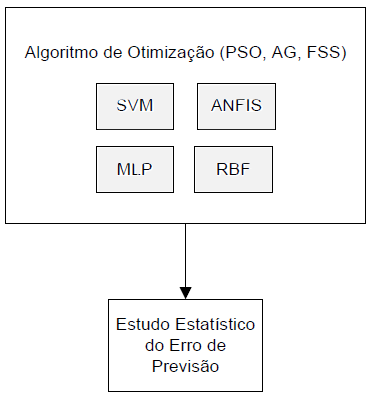
\includegraphics[width=.45\textwidth]{image/MetodologiaDissertacao2.png}
	\caption{Esquema de Seleção da Melhor Rede Neural Artificial.s}
	\label{fig:method2}
\end{figure}

Em quinto lugar, um teste de validação dos resultados é realizado para verificar a eficiência dos modelos baseados em redes neurais artificiais em relação aos modelos de estado da arte em análise de riscos, tais como os modelos baseados em Simulação de Monte Carlo, Análise PERT, Modelo de Regressão Linear Múltipla, Modelo de Regressão em Árvore. Como não existe estudos anteriores para a estimativa do impacto para essa base de dados, os dois últimos modelos de regressão linear foram considerados como linha de base, por serem modelos mais simples. Os dois últimos modelos foram implementados e também são avaliados quanto ao erro na previsão.

As ferramentas utilizadas nesse estudo são Weka, Matlab, o Excel e o programa R. Nessas ferramentas existem bibliotecas de programas que implementam os modelos de regressão linear utilizados e as redes neurais utilizadas. No Excel implementamos a Análise PERT e a Simulação de Monte Carlo.

A seleção do melhor modelo é feita em termos da precisão na estimativa dos impactos dos riscos. É difícil obter uma métrica representativa da precisão de um modelo, no entanto, Engelbrecht \cite{engelbrecht2007computational} e Saxena \cite{saxena2012software} sugerem que a Raiz do Erro Médio Quadrático (REMQ) seja uma medida conveniente e aplicável para a maioria dos problemas. A precisão, nesse caso, significa o grau de proximidade de uma saída calculada para a esperada. A REMQ é representada pela Equação \ref{eq:RMSE}:

\begin{equation}\label{eq:RMSE}
    REMQ= \sqrt[2]{\frac{1}{n}\sum_{i=1}^{n} (e_i)^2} ,
\end{equation}
onde $e_i=f_i - y_i$, $f_i$ é o resultado calculado, $y_i$ é o resultado esperado e $n$ é o número de tuplas de dados.
%where $e_i=f_i - y_i$, $f_i$ is the calculated outcome, $y_i$ is the expected outcome and $n$ is the number of data pairs.

Todas as técnicas estudadas nesse trabalho estimam a saída para o impacto de riscos, a REMQ é calculada trinta vezes para cada abordagem e um Teste Estatístico de Wilcoxon Não-pareado \cite{siegel1956nonparametric} pode ser necessário para determinar qual é uma abordagem mais precisa para a base de dados (nesse estudo, o PERIL). Esse teste estatístico é utilizado porque não há evidências que as amostras sejam oriundas de uma população normalmente distribuída, como também não há relação de ordem nos valores pertencentes às amostras.
%The eight selected techniques have predicted the outcome to risk impacts. Root Mean Square Error was calculated thirty times for each method. Nevertheless, a Non-paired Wilcoxon Test \cite{siegel1956nonparametric} may be necessary to assert which is a more efficient approach to fit the data set (e.g. PERIL). Non-paired Wilcoxon Test is used because there were no evidence that the samples came from a normally distributed population, either there were no relation between outcomes from different samples.

A validação cruzada \cite{amari1996statistical} é utilizada para evitar a ocorrência de \textit{overfitting} ou \textit{underfitting} durante o treinamento das RNA's. Nesse caso, um treinamento com parada prematura é utilizado para identificar o início do \textit{overfitting}, já que esse método tem provado ser capaz de melhorar a capacidade de generalização da RNA em comparação com o treinamento exaustivo \cite{haykin-1994} \cite{engelbrecht2007computational} \cite{amari1996new}. Portanto, o método de validação cruzada é utilizado para cada abordagem, com exceção da Simulação de Monte Carlo e Análise PERT, por promover uma maior capacidade de generalização. Quando se adota o uso da validação cruzada, é necessário o particionamento da base de dados em três partes: conjunto de treinamento, conjunto de validação cruzada e conjunto de testes. O conjunto de treinamento é utilizado na fase de treinamento das RNA's, momento em que o aprendizado ocorre. O conjunto de validação cruzada é processado no mesmo tempo junto com o conjunto de treinamento e determina a parada no treinamento. Já o conjunto de testes, é utilizado para produzir a métrica de precisão do modelo (REMQ).
%Furthermore, cross-validation \cite{amari1996statistical} must be used to avoid the occurrence of overfitting of data training. For instance, \textit{early stopping} training was used to identify the beginning of overfitting because this method has been proved to be capable of improving the generalization performance of the ANN over exhaustive training \cite{haykin1994neural} \cite{amari1996new}. Therefore, cross-validation method are used for each alternative, excluding Monte Carlo Simulation, to promote higher generalization performance.

Por fim, a previsão do impacto do risco e a definição de um intervalo de confiança para uma amostra do conjunto de treinamento são obtidas utilizando o modelo de previsão mais preciso após os testes de validação. É necessário estabelecer um intervalo de confiança da previsão para que os gerentes de projetos e analistas de risco possam estabelecer o nível de confiança de acordo com a sua necessidade. Afinal de contas, esse é o resultado que eles esperam.

A Figura \ref{fig:method} apresenta um fluxograma com a metodologia estabelecida para esse estudo. O procedimento inicia-se com a seleção da base de dados utilizada como conjunto de dados de entrada, nesse caso o PERIL, e finaliza com a atividade ``Definição do Intervalo de Confiança". Todas as atividades são executadas sequencialmente, exceto as atividades ``Avaliação dos Modelos de Estado da Arte" e ``Seleção da Melhor Rede Neural Artificial" que são executadas paralelamente.

\begin{figure}[h]
	\centering
	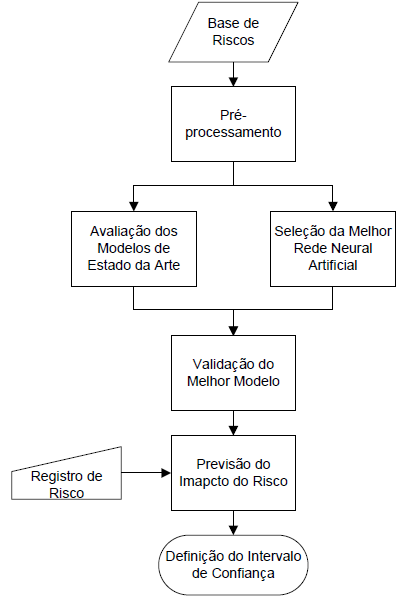
\includegraphics[width=.45\textwidth]{image/MetodologiaDissertacao.png}
	\caption{Fluxograma do estudo realizado.}
	\label{fig:method}
\end{figure}

\section{Base de dados PERIL}
\label{sec:perildataset}

%A better risk management starts identifying potential problems, asserted here as risk factors. The adoption of available methods like: reviewing lessons learned, brainstorming, interviews and specialized judgment are relative efficient alternatives, otherwise in most of situations it involves high costs. A low cost, extensive and accessible proposal is to use Project Experience Risk Information Library (PERIL) database \cite{kendrick2003identifying}. The  PERIL database provides information and experience of other project risk management.
Um melhor gerenciamento de riscos se inicia com a identificação de problemas potenciais, atribuído como fatores de risco. A adoção dos métodos disponíveis como: revisar lições aprendidas, \textit{brainstorming}, entrevistas e opinião especializada são alternativas relativamente eficientes, no entanto, na maioria das situações elas envolvem alto custo. Uma proposta de baixo custo, extensiva e acessível é utilizar a base de dados \textit{Project Experience Risk Information Library}(PERIL) \cite{kendrick2003identifying}. A base de dados PERIL provê informações e experiências de outras gestões de risco de projetos.

%For more than a decade, in Risk Management Workshops, Kendrick have collected anonymous data from hundred of project leaders dealing with their past project problems. He has compiled this data in the PERIL database, which summarizes both a description of what went wrong and the amount of impact it had on each project. The dataset provides a sobering perspective on what future projects may face and is valuable in helping to identify at least some of what might otherwise be invisible risks or black swans \cite{kendrick2003identifying}.
Por mais de uma década, durante \textit{Workshops} de Gerenciamento de Riscos, Kendrick coletou dados anônimos de centenas de líderes de projetos lidando com seus problemas em projetos passados. Ele compilou essas informações na base de dados PERIL, que sumariza tanto uma descrição do que houve de errado quanto o impacto que ele teve em cada projeto. A base provê uma perspectiva preocupante do que projetos futuros podem enfrentar e é valiosa na ajuda para a identificação do que pelo menos poderiam ter sido riscos invisíveis ou \textit{black swans}, isto é, riscos com grande impacto, difíceis de prever e com ocorrência rara \cite{kendrick2003identifying}.

%In projects, the identified risks can be classified as "known", those anticipated during planning, or "unknown", further identified during project execution. The purpose of this dataset is to provide a framework to identify risks, in such a way to increase the number of "known", and decrease the amount of "unknown" risks.
Segundo Kendrick, em projetos, os riscos identificados podem ser classificados como ``conhecidos", aqueles antecipados durante o planejamento, ou ``desconhecidos", identificados futuramente durante a execução do projeto. O propósito dessa base de dados é prover um \textit{framework} para identificar riscos, de modo a aumentar o número de riscos "conhecidos" e diminuir o número de riscos "desconhecidos" \cite{kendrick2003identifying}.

%Some characteristics of PERIL are: 
%\begin{itemize}
%\item the data are not relational, they contain only a small fraction of the tens of thousands projects undertaken by the project leaders from whom they were collected;
%\item they present bias, the information was not collected randomly;
%\item they represent only the most significant risks;
%\item they are worldwide, with a majority from the Americas;
%\item they do not identify opportunities; 
%\item they contain six hundred and forty nine registers, whose relative impact is based on the number of weeks delayed the project schedule;
%\item typical project had a planned duration between six months and one year;
%\item typical staffing was rarely larger than about twenty people.
%\end{itemize}
Algumas características observadas na base de dados PERIL são:
\begin{itemize}
\item Os dados não estão relacionados, eles representam somente uma pequena fração de dezenas de milhares de projetos realizados por líderes de projetos, cujos riscos foram coletados;
\item Apresentam viés, a informação não foi coletada aleatoriamente;
\item Representam somente os riscos mais significativos;
\item Foram coletadas no mundo todo, majoritariamente nas Américas;
\item Não identificam oportunidades; 
\item Contém 772 registros, cujo impacto relativo é baseado no número de semanas de atraso no cronograma;
\item Projetos comuns tiveram um cronograma inicialmente planejado entre seis meses e um ano;
\item Tamanho da equipe raramente maior do que vinte pessoas.
\end{itemize}

%Risk registers are categorized as scope, schedule and resource. Scope is decomposed in change and defect subcategories. Schedule is decomposed in dependency, estimative and delay subcategories. Resources is decomposed in money, outsourcing and people subcategories. One benefit of PERIL is that the author contemplates "black swans": risks with large impact, difficult to predict and with rare occurrence \cite{taleb2001fooled}. 
Os registros de risco são categorizados em escopo, cronograma e recurso. O escopo é decomposto nas subcategorias mudança e defeito. O cronograma é decomposto em dependência, estimativa e atraso. Os recursos são decompostos em dinheiro, \textit{outsourcing} e pessoas. Um benefício da PERIL é que o autor contempla ``\textit{black swans}" que são riscos com grande impacto, difíceis de prever e de rara ocorrência \cite{taleb2001fooled}.

%Kendrick chose to normalize all the quantitative data using only time impact, measured in weeks of project slippage. This tactic made sense in light of today's obsession with meeting deadlines, and it was an easy choice because by far the most prevalent serious impact reported in this data was deadline slip. Focusing on time is also appropriate because among the project triple constraints of scope, time ans cost, time is the only one that's completely out of our control - when it's gone, it's gone \cite{KEND2003BOOK}.
Kendrick decidiu padronizar o impacto usando como métrica o tempo, medido em semanas de atraso no projeto. Essa estratégia faz sentido à luz da obsessão de hoje por cumprimento de prazos e foi uma escolha fácil, pois, de longe, o impacto mais sério relatado nesses dados foi o atraso no prazo. Focar-se em tempo também é apropriado porque entre as restrições triplas de projeto - escopo, tempo e custo -, tempo é o único que está completamente fora de nosso controle. Afinal, o tempo sempre passa e quando não se é utilizado, não é possível voltar atrás \cite{KEND2003BOOK}.

%\begin{table}[h]
%\caption{Raw project numbers in the PERIL database}\label{tab:peril_numbers} \centering
%\begin{tabular}{|l|c|c|c|c|}
% \hline
% \multicolumn{1}{|c|}{} &Americas &Asia &Europe/Middle East &Total \\
% \hline
%  IT/Solution Project & 256 & 57 & 18 & 331 \\
%  Product Development Project & 224 & 66 & 28 & 318 \\
% \hline
%  \textbf{Total} & \textbf{480} & \textbf{123} & \textbf{46} & \textbf{649} \\
% \hline
%\end{tabular}
%\end{table}
\begin{table}[h]
\caption{Número bruto de projetos no PERIL}\label{tab:peril_numbers} \centering
\begin{tabular}{|l|c|c|c|c|}
 \hline
 \multicolumn{1}{|c|}{} & Américas & Ásia & Europa/Oriente Médio & Total \\
 \hline
  Projeto de TI/Soluções & 280 & 77 & 37 & 394 \\
  Projeto de Des. de Produto & 249 & 86 & 43 & 378 \\
 \hline
  \textbf{Total} & \textbf{529} & \textbf{163} & \textbf{80} & \textbf{772} \\
 \hline
\end{tabular}
\end{table}

Na Tabela \ref{tab:peril_numbers}, apresenta-se o número de projetos em TI e de desenvolvimento de produtos nas Américas, Ásia e Europa.

\begin{table}[h]
\caption{Impacto total de projetos pelas causas-raiz de categorias e subcategorias \cite{KEND2003BOOK}}\label{tab:peril_pareto} \centering
\begin{tabular}{|l|c|c|c|c|}
 \hline
 Subcat. & & & Impacto & Impacto \\
 Causas-raiz & Definição & Casos & Cumul. & Médio \\
  &  &  & (sem.) & (sem.) \\
 \hline
  Escopo: & Revisão no escopo &  &  &  \\
  Mudanças & durante o projeto & 177 & 1460 & 8,2 \\
 \hline
  Recurso: &  &  &  &  \\
  Pessoas & Problemas de relacionamento interno & 123 & 706 & 5,7 \\
 \hline
  Escopo: & Falha em alcançar  &  &  &  \\
  Defeito & requisitos de entrega & 93 & 654 & 7,0 \\
 \hline
  Cronograma: & Atraso devido a fatores &  &  &  \\
  Atrasos & sob o controle do projeto & 102 & 509 & 5,0 \\
 \hline
  Cronograma: & Durações inadequadas alocadas &  &  &  \\
  Estimativas & para atividades do projeto & 49 & 370 & 7,6 \\
 \hline
  Recurso: &  &  &  &  \\
  \textit{Outsourcing} & Problemas de relacionamento externo & 47 & 316 & 6,7 \\
 \hline
  Cronograma: & Atraso no projeto devido &  &  &  \\
  Dependências & a fatores externos & 41 & 262 & 6,4 \\
 \hline
  Escopo: &  &  &  &  \\
  Mudanças & Financiamento insuficiente & 17 & 228 & 13,4 \\
 \hline
\end{tabular}
\end{table}
%\begin{table}[h]
%\caption{Total project impact by root-cause categories and subcategories \cite{KEND2003BOOK}}\label{tab:peril_pareto} \centering
%\begin{tabular}{|l|c|c|c|c|}
 %\hline
 %Root-Cause & & &Cumulative &Average \\
 %Subcategories &Definition &Cases &Impact(weeks) &Impact(weeks) \\
 %\hline
 % Scope: & Revision made to scope &  &  &  \\
 % Changes & during the project & 177 & 1,460 & 8.2 \\
 %\hline
 % Resource: &  &  &  &  \\
 % People & Issues arising from internal staffing & 123 & 706 & 5.7 \\
 %\hline
 % Scope: & Failure to meet deliverable &  &  &  \\
 % Defects & requirements & 93 & 654 & 7.0 \\
 %\hline
 % Schedule: & Project slippage due to factors &  &  &  \\
 % Delays & under the control of the project & 102 & 509 & 5.0 \\
 %\hline
 % Schedule: & Inadequate durations allocated &  &  &  \\
 % Estimates & to project activities & 49 & 370 & 7.6 \\
 %\hline
 % Resource: &  &  &  &  \\
 % Outsourcing & Issues arising from external staffing & 47 & 316 & 6.7 \\
 %\hline
 % Schedule: & Project slippage due to factors &  &  &  \\
 % Dependencies & outside the project & 41 & 262 & 6.4 \\
 %\hline
  %Scope: &  &  &  &  \\
  %Changes & Insufficient project funding & 17 & 228 & 13.4 \\
% \hline
%\end{tabular}
%\end{table}

A Tabela \ref{tab:peril_pareto} apresenta o número de casos, o impacto cumulativo e médio em semanas para cada categoria e sub-categoria de causa-raiz, além do significado de cada subcategoria.

Uma desvantagem dessa base de dados é que ela somente contabiliza riscos que tiveram impacto negativo no projeto. As oportunidades não foram identificadas e analisadas nesse estudo. No entanto, um dos grandes benefícios é que o autor apresenta alguns riscos como \textit{black swans} \cite{KEND2003BOOK}, então utilizando a PERIL responde-se a primeira questão dessa pesquisa. Se o risco tiver impacto negativo é conhecido como catástrofe, ao passo que, se tiver impacto positivo é conhecido como recompensa.
%A disadvantage of this database is that it only accounts for risks that negatively impact on the project. The opportunities were not identified and maximized in that study. However, A major benefit is that the author presents some risks as black swans \cite{KEND2003BOOK}: representing the idea of risks with broad impact, hard to predict and rare to occur. If the risk has negative impact, is known as a catastrophe, whereas, if you have positive impact, is known as a reward.

\subsection{\textit{Black Swans}}

%Calling some risks "black swans" has been popularized of late by the writings of Nassim Nicholas Taleb \cite{taleb2001fooled}. The notion of a "black swan" originated in Europe before there was much knowledge of the rest of the world. Because all the swans observed in Europe were white, a black swan was deemed impossible. It came as something of a shock when a species of black swans was later discovered in Australia. This realization gave rise to the metaphorical use of the term "black swan" to describe something erroneously believed to be impossible.
Denominar alguns riscos como \textit{black swans} têm sido popularizado desde os textos de Nassim Nicholas Taleb \cite{taleb2001fooled}. A noção de \textit{black swan} originou-se na Europa antes de ser popularizada pelo Mundo. Já que todos os cisnes observados na Europa eram brancos, um cisne negro era considerado impossível de existir. Porém, foi como um choque quando uma espécie de cisne negro foi descoberta na Austrália. Esse fato deu origem ao uso metafórico do termo \textit{black swan} para descrever algo erroneamente acreditado ser impossível.

%Taleb's concept of "black swan" is a large-impact, hard-to-predict, rare event. It is nonetheless applicable to project risk management. In projects, it is common for project leaders to discount major project risks because they are estimated to have extremely low probabilities. But these risks do occur - The PERIL database is full of them - and the severity of problems they cause means that ignoring them can be unwise. When these risks do occur, the same project managers who initially dismissed them come to perceive them as much more predictable - sometimes even inevitable \cite{KEND2003BOOK}.
O conceito de Taleb acerca de \textit{black swan} define-o como um evento raro, difícil de prever e de grande impacto. Mas não deixa de ser aplicável a gestão de risco do projeto. Nos projetos, é comum que os líderes de projeto descartem os principais riscos do projeto, devido as suas probabilidades serem extremamente baixas. No entanto, esses riscos ocorrem - a PERIL é cheia deles - e a severidade dos problemas que eles causam significa que ignorá-los pode ser imprudente. Quando esses riscos ocorrem, o mesmo gerente de projetos que inicialmente os negaram começam a percebê-los como muito mais previsíveis - às vezes até mesmo inevitáveis \cite{KEND2003BOOK}.

%In PERIL database, there are 127 cases representing the most schedule slippage. As the database shows, these most damaging risks are not as rare as might be thought, and they need not be so difficult for project managers to predict if they get appropriate attention in the risk management process \cite{KEND2003BOOK}. In many situations, the most difficult task is to identify and estimate "black swans" due to its characteristic: emergent, unexpected, unpredictable and extreme impact events. Therefore, "black swans" also will be included in this study.
Na PERIL, há cento e vinte e sete casos representando os maiores atrasos no cronograma. Como a base de dados mostra, estes riscos mais danosos não são tão raros quanto devem ser pensados, e não devem ser tão difíceis de ser previstos por gerentes se eles dedicarem a atenção apropriada para o processo de gerenciamento de riscos \cite{KEND2003BOOK}. Em muitas situações, a tarefa mais difícil é identificar e estimar \textit{black swans} devido a sua característica: emergente, inesperado, imprevisível e com alto impacto. Portanto, \textit{black swans} também são considerados nesse estudo.

\section{Pré-processamento dos Dados}
\label{sec:datapreprocessing}

%PERIL contains nominal and numeric values. So, nominal variables were expressed through binary variables. In that point, it is used fifteen binaries variables to represent nine nominal variables. Second, impact which represents the real output, are integer numbers. It has been noticed that impact probability distribution function fits with log-normal, gamma functions. Therefore, it was done a gamma data normalization \cite{han2006data}.
PERIL contém valores nominais e numéricos. As variáveis nominais foram expressas através de variáveis binárias. Nesse estudo, utilizam-se doze variáveis binárias para representar as variáveis nominais. O impacto que representa a saída esperada, são números inteiros. Foi observado que a função de distribuição de probabilidade do impacto ajusta-se às funções log-normal e gamma. Portanto, foi realizada uma normalização gamma \cite{han2006data}. A seleção das variáveis mais significativas para o estudo foi realizada após o resultado da análise promovida pelo algoritmo \textit{Random Forest} proposto no livro de Luís Torgo \cite{torgo2003data}.

%Figure \ref{fig:input16} e \ref{fig:input712} introduced input variables in histograms. All data are binary values represented by bar graphs, that means the number of occurrences for each value interval. Figure \ref{fig:impacthistogram} presents gamma normalized real outcome from PERIL in a histogram. A shape of the distribution fitting function is also presented in a curve under the histogram.
A Figura \ref{fig:input16} e \ref{fig:input712} apresentam os histogramas das variáveis de entrada. Todos os dados encontram-se binarizados como pode ser observado nos gráficos em barras, que contém o número de ocorrências para cada intervalo de valores. A Figura \ref{fig:impacthistogram} apresenta a saída normalizada pela função gamma para a PERIL num histograma. A forma da função de distribuição de probabilidade é exibida como uma curva sobre o histograma.

%\begin{figure}[h]
%  \vspace{-0.2cm}
%  \centering
%  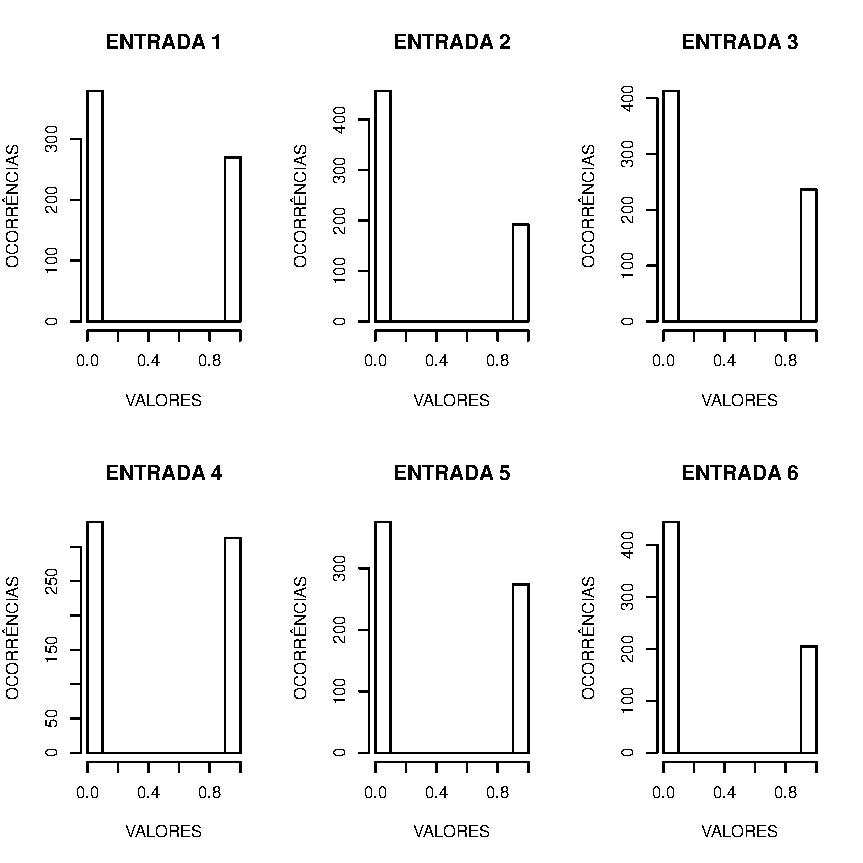
\includegraphics[width=0.7\columnwidth]{image/input1_6.pdf}
%  \caption{First six input variables}
%  \label{fig:input16}
%\end{figure}
\begin{figure}[h]
  \vspace{-0.2cm}
  \centering
  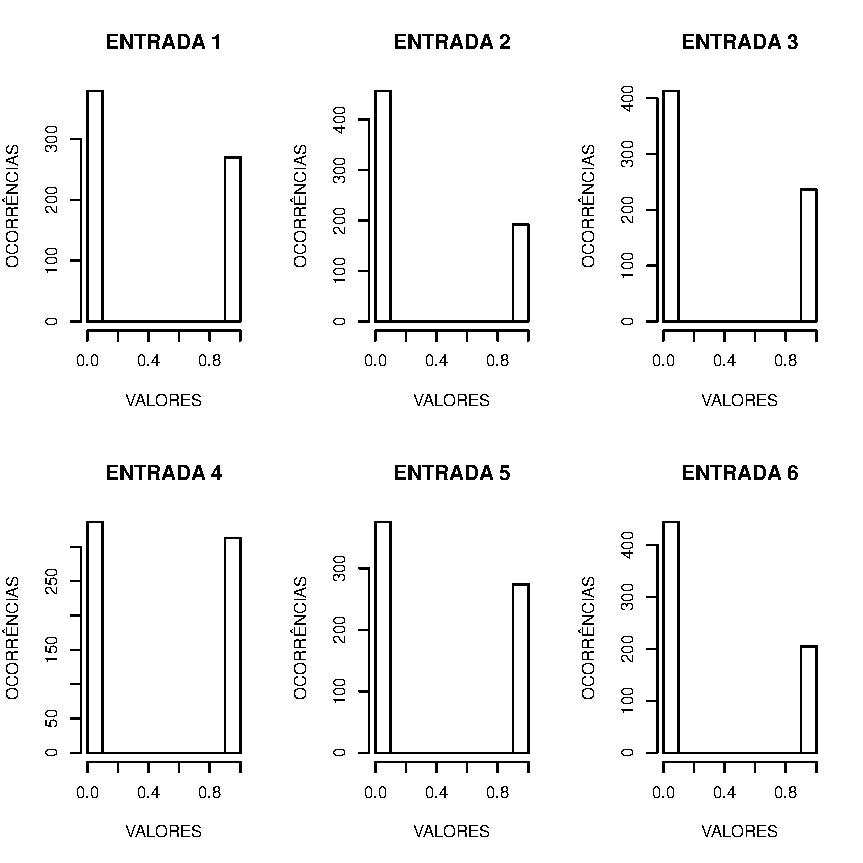
\includegraphics[width=0.7\columnwidth]{image/input1_6.pdf}
  \caption{Primeiras seis variáveis de entrada.}
  \label{fig:input16}
\end{figure}

%\begin{figure}[h]
%  \vspace{-0.2cm}
%  \centering
%  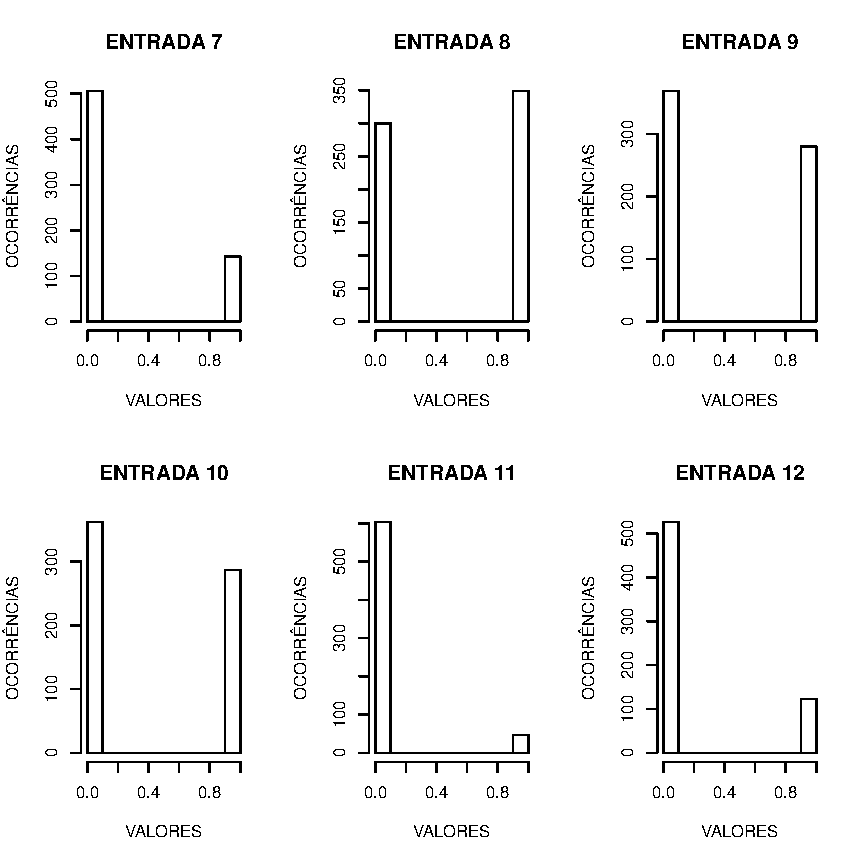
\includegraphics[width=0.7\columnwidth]{image/input7_12.pdf}
%  \caption{Last six input variables}
%  \label{fig:input712}
%\end{figure}
\begin{figure}[h]
  \vspace{-0.2cm}
  \centering
  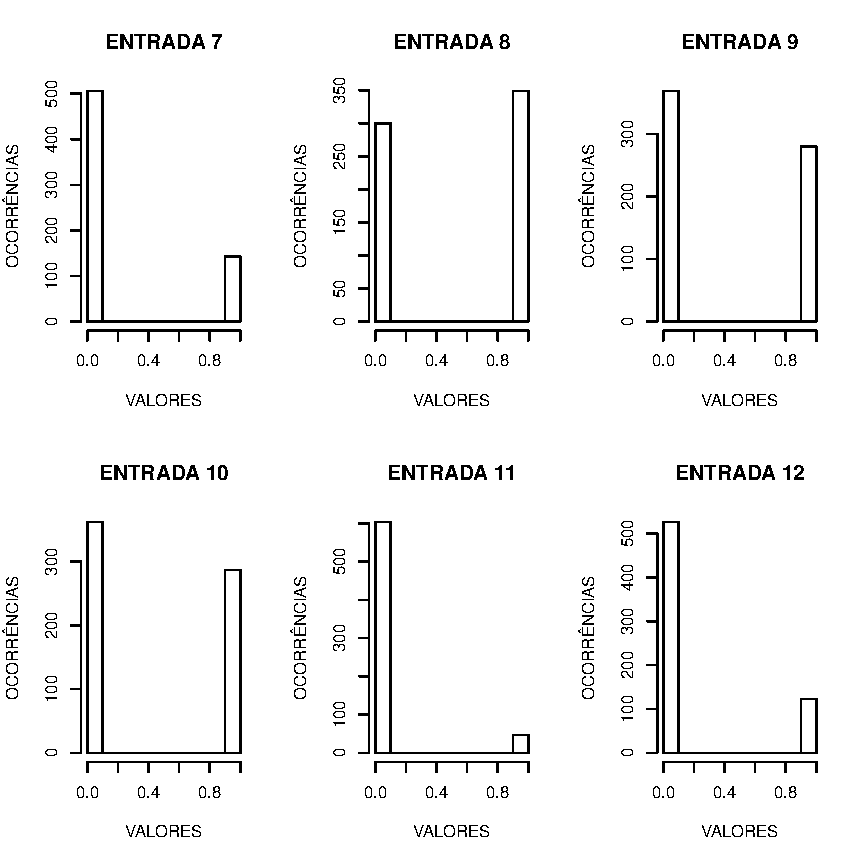
\includegraphics[width=0.7\columnwidth]{image/input7_12.pdf}
  \caption{Últimas seis variáveis de entrada.}
  \label{fig:input712}
\end{figure}

%\begin{figure}[h]
%  \vspace{-0.2cm}
%  \centering
%  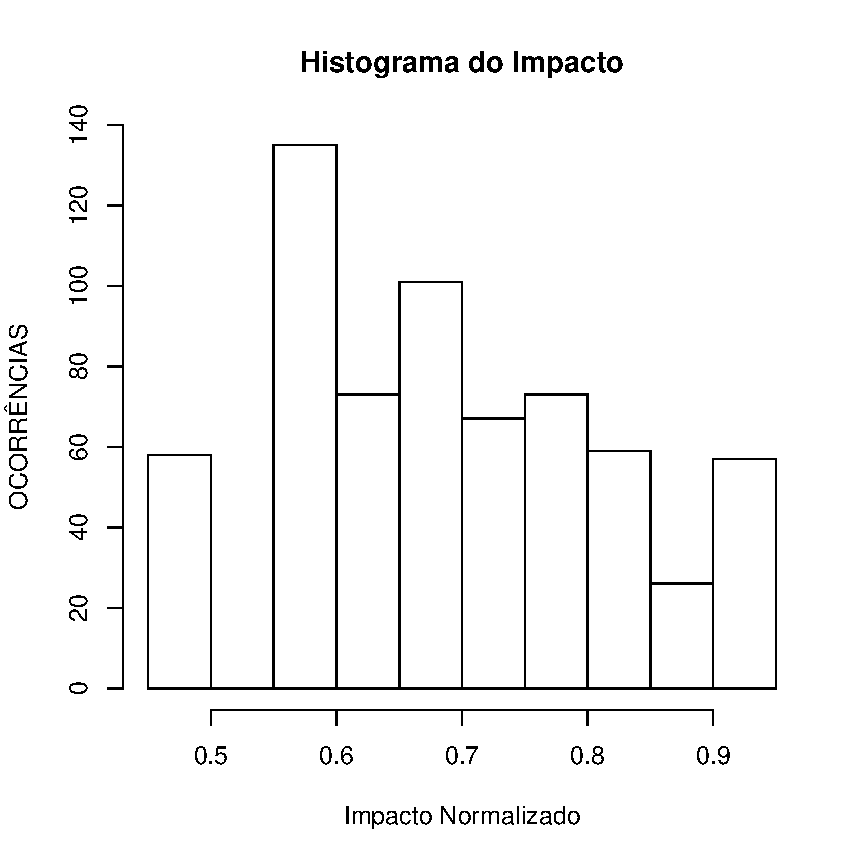
\includegraphics[width=0.5\columnwidth]{image/impact_histogram.pdf}
%  \caption{Histogram of impact and shape of the distribution fitting function}
%  \label{fig:impacthistogram}
%\end{figure}
\begin{figure}[h]
  \vspace{-0.2cm}
  \centering
  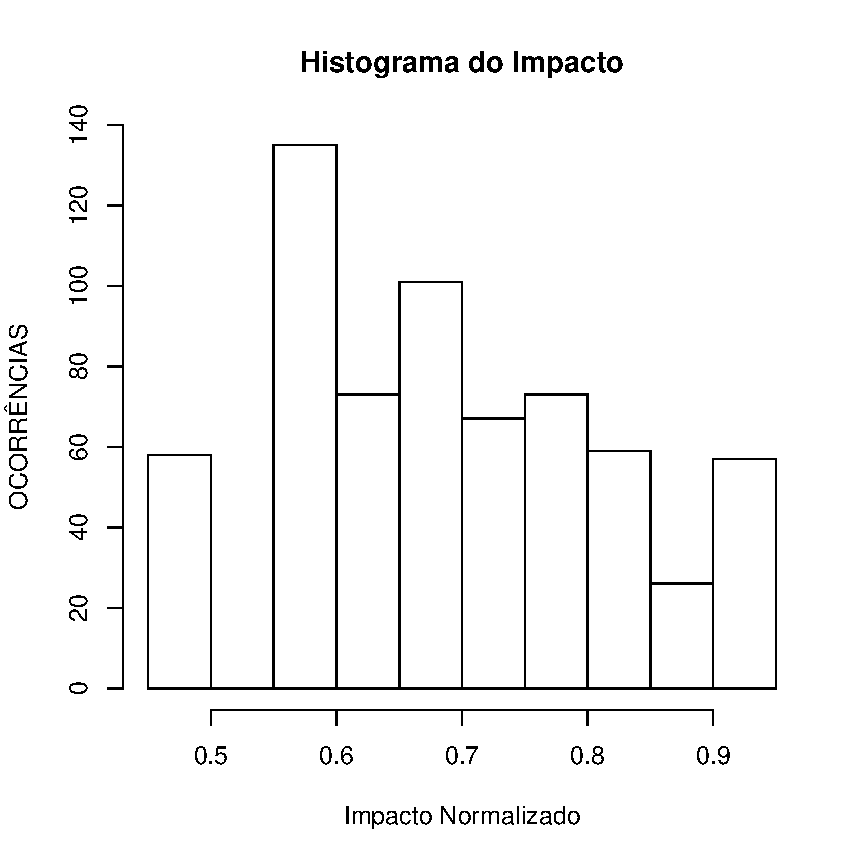
\includegraphics[width=0.5\columnwidth]{image/impact_histogram.pdf}
  \caption{Histograma do impacto e forma da função de distribuição de ajuste.}
  \label{fig:impacthistogram}
\end{figure}

%For our purpose, PERIL was split into three disjoint subsets - training, cross-validation and test subsets, corresponding to fifty, twenty-five and twenty five percent of the dataset, respectively. \textit{Split-sample} cross-validation method was used for MLRM and RTM models. Whereas \textit{early stopping} and \textit{split-sample} cross-validation methods were combined and used for MLP, SVM, RBF and ANFIS training \cite{priddy2005artificial}.
Para o nosso objetivo, PERIL foi dividida em três subconjuntos disjuntos - treinamento, validação cruzada e teste, correspondendo a cinquenta, vinte e cinco porcento e o restante da base de dados, respectivamente. O método de validação-cruzada com divisão de amostras foi utilizado tanto para o MRLM e o MRA quanto para o MLP, SVM, RBF e o ANFIS; sendo que para os últimos o método da parada prematura também foi utilizada no treinamento \cite{priddy2005artificial}.

\section{Modelos de Estado da Arte}
\label{sec:models}

Nesta seção, são descritas as configurações adotadas para a experimentação dos modelos de estado da arte.

\subsection{Simulação de Monte Carlo}

%MCS technique used the entire dataset in order to increase the performance prediction. It was filtered only the possible real outcomes to generate the calculated outcome. Towards this decision, we have reduced prediction issues and have improved its performance.
A Simulação de Monte Carlo utilizou a base de dados completa com o objetivo de aumentar o desempenho do modelo durante a previsão. Além disso, foram filtradas somente as saídas possíveis para uma dada entrada para que uma nova saída pudesse ser calculada, através dessa configuração, o desempenho da estimativa do impacto dos riscos foi melhorado. Já que, a SMC é um método estatístico, a previsão de valores a partir de uma amostra pouco representativa como ocorre quando não se filtram somente as saídas possíveis geram previsões mais errôneas.

\subsection{Análise PERT}

A Análise PERT também utilizou a base de dados completa e somente as saídas possíveis para uma determinada entrada foi utilizada no cálculo da nova saída, tal qual a SMC. A partir dessa configuração o resultado desse modelo foi melhorado, em comparação com o cenário em que a base de dados não foi filtrada.

\section{Modelos de Regressão Linear}

Nesta seção, são descritas as configurações adotadas para a experimentação com os modelos de regressão linear. 

%The source code of MLR models were adapted from Torgo \cite{torgo2003data} in order to perform linear regression model training, cross-validation, outcome prediction and MAE evaluation. MLR and RTM models were analyzed statistically to define the baseline linear regression model for further analysis.
O código-fonte dos modelos de regressão linear foram adaptados de Torgo \cite{torgo2003data} para realização do treinamento, validação cruzada, teste e avaliação da Raiz do Erro Médio Quadrático. Os modelos MRLM e MAR foram comparados estatisticamente para que se pudesse definir um modelo de regressão linear padrão para estudos futuros com a base de dados correspondente.

Um estudo com esses modelos de regressão linear são necessários porque não há um estudo base para a estimativa de impactos de risco utilizando a PERIL. Portanto, durante os experimentos, a avaliação do melhor modelo de regressão linear tem como objetivo definir um limite superior de valores da REMQ. Isso significa que os modelos que obtiverem erros acima desse limite superior são insatisfatórios.

\subsection{Modelo de Regressão Linear Múltipla}

O MRLM é um  modelo de regressão linear mais simples para a estimativa do impactos dos riscos apresentados na PERIL. Após a otimização do Modelo de Regressão Linear através da seleção das melhores variáveis de entrada utilizando o critério \textit{Akaike Information Criterion}(AIC) sete das onze variáveis foram selecionadas, além do termo independente.

\subsection{Modelo de Regressão em Árvore}

O modelo MRA constrói uma árvore de classificação das variáveis de entrada, podendo não ser necessário utilizar todas as variáveis de entrada para a construção do modelo. Ele tenta obter erros de previsão menores que o MRLM através da seleção das variáveis de entrada que têm maior correlação linear com a saída. Na Seção \ref{cap:experiments}, três modelos de árvore de regressão foram analisados com o modelo de regressão linear múltipla.

\section{Otimização por Enxame de Partículas}

Para o PSO, os parâmetros descritos na Tabela \ref{tab:pso_configuration} foram utilizados. Esses parâmetros foram definidos experimentalmente. A variação do PSO utilizada é aquela que implementa o coeficiente de constrição de Clerk \cite{clerc1999swarm}, como definido no início desse capítulo.

\begin{table}[h]
\caption{Parâmetros do PSO.}\label{tab:pso_configuration} \centering
\begin{tabular}{|c|c|}
  \hline
  Parameter & Value \\
  \hline
  Coeficiente Cognitivo & 2,05 \\
  \hline
  Coeficiente Social & 2,05 \\
  \hline
  Fator de Inércia & 0,8 \\
  \hline
  Número de partículas & 30 \\
  \hline
  Número de ciclos & 600 \\
  \hline
\end{tabular}
\end{table}

Cada partícula no PSO representa uma configuração candidata. A função de avaliação das partículas é a REMQ de trinta avaliações da rede neural artificial analisada cujos parâmetros são cada partícula. Os parâmetros das redes MLP, SVM e RBF são determinados após a execução desse algoritmo.

\section{Redes Neurais Artificiais}
\label{sec:rnas}

Nesta seção, são descritas as configurações das redes neurais artificiais utilizadas nesse estudo.

\subsection{MLPs}

%A three layered back-propagation MLP model was established to model risk impact predictor. That model consists of one input layer, one hidden layer, and one output layer. The input layer had thirteen neurons, which represent the twelve independent variables plus the bias. The output layer has one neuron, which represents the single impact outcome. The transfer function in hidden and output layer was sigmoid-logistic. The architecture of the MLP is demonstrated in Figure \ref{fig:mlpmodelstudy}.
Algumas variações do modelo da MLP foram utilizadas nesse estudo. Diversos parâmetros podem ser alterados tais como a quantidade de camadas escondidas, o número de neurônios escondidos em cada camada escondida, a taxa de aprendizado, o momento, o número máximo de ciclos de treinamento e a regra de aprendizado. Um modelo MLP utilizado nesse estudo é apresentado na Figura \ref{fig:mlp_example}. Nesse modelo tem-se dez neurônios escondidos na única camada escondida.

\begin{figure}[!h]
  \vspace{-0.2cm}
  \centering
  \def \svgwidth{0.55\columnwidth}
  \input{image/mlp.pdf_tex}
  \caption{Um modelo MLP utilizado no estudo.}
  \label{fig:mlp_example}
\end{figure} 

%The number of neurons in the hidden layer and other paramenters were determined by trial and error, a fast approach aiming to achieve a more accurate performance of MLP. For the analysis, the maximum training epochs has been set at six hundreds.
A quantidade de camadas escondidas estudadas foram uma e duas camadas. O número de neurônios na(s) camada(s) escondida(s), a taxa de aprendizado e o momento foram determinados por um algoritmo de otimização como o PSO para aumentar a precisão na estimativa de erros. Para as análises, o número máximo de ciclos de treinamento foi configurado para seiscentos.

%Learning rate, momentum and neurons in hidden layer varied from values presented in Table \ref{tab:mlp_configuration_investigation}. A better parameters configuration solution is shown in Table \ref{tab:mlp_best_configuration}. Figure \ref{fig:mlpmodelstudy} presents MLP model with the better configuration for PERIL. The model contains ten neurons in hidden layer.
A taxa de aprendizado, o momento e a quantidade de neurônios na camada escondida variam de acordo com os valores apresentados na Tabela \ref{tab:mlp_configuration_investigation}.

%\begin{table}[h]
%\caption{Parameters intervals to MLP model.}\label{tab:mlp_configuration_investigation} \centering
%\begin{tabular}{|c|c|c|}
%  \hline
%  Parameter & Min. Value & Max. Value \\
%  \hline
%  Momentum & 0.1 & 0.9 \\
%  \hline
%  Learning rate & 0.1 & 0.9 \\
%  \hline
%  Hidden Neurons & 1 & 100 \\
%  \hline
%\end{tabular}
%\end{table}
\begin{table}[h]
\caption{Intervalos de parâmetros para a MLP.}\label{tab:mlp_configuration_investigation} \centering
\begin{tabular}{|c|c|c|}
  \hline
  Parâmetros & Valor Mínimo & Valor Máximo \\
  \hline
  Momento & 0,1 & 0,9 \\
  \hline
  Taxa de Aprendizado & 0,1 & 0,9 \\
  \hline
  Neurônios Cam. Escondida & 1 & 100 \\
  \hline
\end{tabular}
\end{table}

Por fim, as regras de aprendizado utilizadas nesse estudo são \textit{Backpropagation}, Levenberg-Marquardt, BFGS Quasi-Newton, \textit{Resilient Backpropagation}, \textit{Polak-Ribiére Conjugate Gradient}, Gradiente Conjugado Escalonado e \textit{One Step Secant}.

Em particular, uma MLP, chamada ``MLPRegressor", que tem uma camada escondida e cuja regra de aprendizado tem o objetivo de minimizar o erro médio quadrático mais uma penalidade quadrática através do método BFGS Quasi-Newton teve um melhor desempenho que as demais variações.

\subsection{SVM}

%RegSMOImproved is the optimization algorithm and PolyKernel is the kernel function as described in \cite{Shevade1999}. 
O algoritmo SVM para regressão utilizado é o SMOReg. Nesse algoritmo RegSMOImproved é o algoritmo de otimização e PolyKernel é a função de kernel como descrito em \cite{Shevade1999}. O pseudo-código para esse algoritmo é apresentado no Algoritmo \ref{alg:pseudocodigoSVM}.


\begin{algorithm}[H]
%\SetAlgoLined
\label{alg:pseudocodigoSVM}
\begin{verbatim}
Begin
     peril <- read_file();
     peril_train <- partition(peril, 0, 50);
     peril_crossvalidation <- partition(peril, 50, 75);
     peril_test <- partition(peril, 75, 100);
     smo <- SMOReg();
     options <- [peril_train, peril_crossvalidation, 
                 RegSMOImproved, PolyKernel]
     SMOReg.runClassifier(smo, options);
     for instance in peril_test:
          calculated <- smo.classifyInstance(instance);
          wished <- instance.classValue();
          REMQ <- REMQ + (wished - calculated)^2
     end
     n <- peril_test.size();
     REMQ <- REMQ/n;
     REMQ <- sqrt(REMQ);
 End
\end{verbatim}     
\caption{Algoritmo do SVM}
\end{algorithm}
\bigskip

%In Algorithm \ref{code:svm}, we read data on file, split data into training, cross-validation and testing subsets, instantiates SMOReg SVM regression model, run model training, generates a calculated outcome, get the correspondent real output in PERIL and calculate MAE.
No Algoritmo \ref{alg:pseudocodigoSVM}, os dados são lidos a partir de um arquivo, dividido nos subconjuntos treinamento, validação cruzada e teste. O modelo de regressão SMOReg é instanciado, o treinamento do modelo é executado, a saída calculada é gerada e é calculado o REMQ a partir da saída real e da saída calculada. Esse algoritmo é utilizado como a função de otimização para o algoritmo de otimização por enxame.

\subsection{RBF}

A rede neural RBF utilizada é a RBFRegressor. Ela minimiza o erro quadrático através do método BFGS. Os centros iniciais das gaussianas são encontrados utilizando SimpleKMeans, um algoritmo que implementa K-Médias. O sigma inicial é configurado para a maior distância entre qualquer centro e o vizinho mais próximo no conjunto de centros. O parâmetro de cume é usado para penalizar o tamanho dos pesos na camada de saída, o qual implementa uma combinação linear simples. O número de funções de base pode também ser especificado. Para esse estudo somente um sigma global é utilizado para todas as funções de base. O pseudo-código para esse algoritmo é apresentado no Algoritmo \ref{alg:pseudocodigoRBF}.

\begin{algorithm}[H]
%\SetAlgoLined
\label{alg:pseudocodigoRBF}
\begin{verbatim}
 Begin
     peril <- read_file();
     peril_train <- partition(peril, 0, 50);
     peril_crossvalidation <- partition(peril, 50, 75);
     peril_test <- partition(peril, 75, 100);
     rbf <- RBFRegressor();
     options <- [peril_train, peril_crossvalidation, peril_test]
     RBFRegressor.runClassifier(rbf, options);
     for instance in peril_test:
          calculated <- rbf.classifyInstance(instance);
          wished <- instance.classValue();
          REMQ <- REMQ + (wished - calculated)^2
     end
     n <- peril_test.size();
     REMQ <- REMQ/n;
     REMQ <- sqrt(REMQ);
 End
\end{verbatim}
\caption{Algoritmo do RBF}
\end{algorithm} 
\bigskip

%In Algorithm \ref{code:svm}, we read data on file, split data into training, cross-validation and testing subsets, instantiates SMOReg SVM regression model, run model training, generates a calculated outcome, get the correspondent real output in PERIL and calculate MAE.
No Algoritmo \ref{alg:pseudocodigoRBF}, os dados são lidos a partir de um arquivo, dividido nos subconjuntos treinamento, validação cruzada e teste. O modelo de regressão SMOReg é instanciado, o treinamento do modelo é executado, a saída calculada é gerada e a REMQ é obtida a partir das saídas real e calculada. Esse algoritmo é utilizado como a função de otimização para o algoritmo de otimização por enxame.

\subsection{ANFIS}

O ANFIS é um sistema \textit{neuro-fuzzy} desenvolvido por Sugeno \cite{jang1997neuro}. Ele utiliza um algoritmo de aprendizado híbrido para identificar parâmetros do sistema de inferência \textit{fuzzy} Sugeno. Ele aplica uma combinação do método dos mínimos quadrados e o método do gradiente descendente \textit{backpropagation} para o treinamento dos parâmetros da função de pertinência do sistema de inferência \textit{fuzzy}. O sistema de inferência \textit{fuzzy} utilizado foi o ``genfis2", já que há um número grande de variáveis de entrada. O pseudo-código para esse algoritmo é apresentado no Algoritmo \ref{alg:pseudocodigoANFIS}.

\begin{algorithm}[H]
%\SetAlgoLined
\label{alg:pseudocodigoANFIS}
\begin{verbatim}
 Begin
     inputs = csvread(peril,0,0,[0,0,648,10])
     targets = csvread(peril,0,11)
     tData = [inputs targets];
     in_fis = genfis2(inputs,targets, 0.7);
     trainOpts = [100,0.1,0.01,0.9,1.1]
     displayOpts = [1,1,1,1];
     chkData = []
     [fis,error,stepsize,chkFis,chkErr] = 
          anfis(tData,in_fis,trainOpts,displayOpts,
          chkData,1);
     for err in error:
          REMQ <- REMQ + (err)^2
     end
     n <- peril.size();
     REMQ <- REMQ/n;
     REMQ <- sqrt(REMQ);
 End
\end{verbatim}
\caption{Algoritmo do ANFIS}
\end{algorithm}
\bigskip

%In Algorithm \ref{code:svm}, we read data on file, split data into training, cross-validation and testing subsets, instantiates SMOReg SVM regression model, run model training, generates a calculated outcome, get the correspondent real output in PERIL and calculate MAE.
No Algoritmo \ref{alg:pseudocodigoANFIS}, os dados de entrada e saída são lidos a partir de um arquivo. O sistema de inferência \textit{fuzzy} é instanciado, o treinamento do modelo é executado, o erro é gerado e a REMQ é obtida a partir das saídas real e calculada. Esse algoritmo é utilizado como a função de otimização para o algoritmo de otimização por enxame.

\pagebreak